\documentclass{article}
\usepackage{KJN}
\usepackage{a4wide,changebar}
\usepackage[numbered,framed]{mcode}

\title{Introduction to Vision and Robotics: Assignment 1}
\author{Chris Swetenham: Student Num, Daniel Mankowitz: S1128165}
\date{3/11/2011}

\begin{document}
\maketitle

\section{Introduction}
\label{sec:introduction}
%An overview of the main ideas used in the approach


\section{Methods}
\label{sec:methods}
%Describe the vision techniques used

%Detail how these ideas were implemented

%Describe the structure of the code

%How each part is meant to work

%Justify design decisions where appropriate

\subsection{Linking Algorithm}
\label{sec:linking}
The linking algorithm is used to link together detections of a single robot in consecutive frames. Since the images provided in the dataset are RGB, the linking algorithm has been implemented to run on each of the three colour channels respectively. 

The algorithm is shown in \figref{fig:link}. Initially, the image on the $k^{th}$ iteration will have been split into three colour channels of red, green and blue respectively. Each colour channel is represented as a separate image. The robots in each colour channel will have been identified and their optimum bounding boxes need to be calculated. These images are fed into the linking algorithm. 


\begin{figure}[h!] 
  \centering
    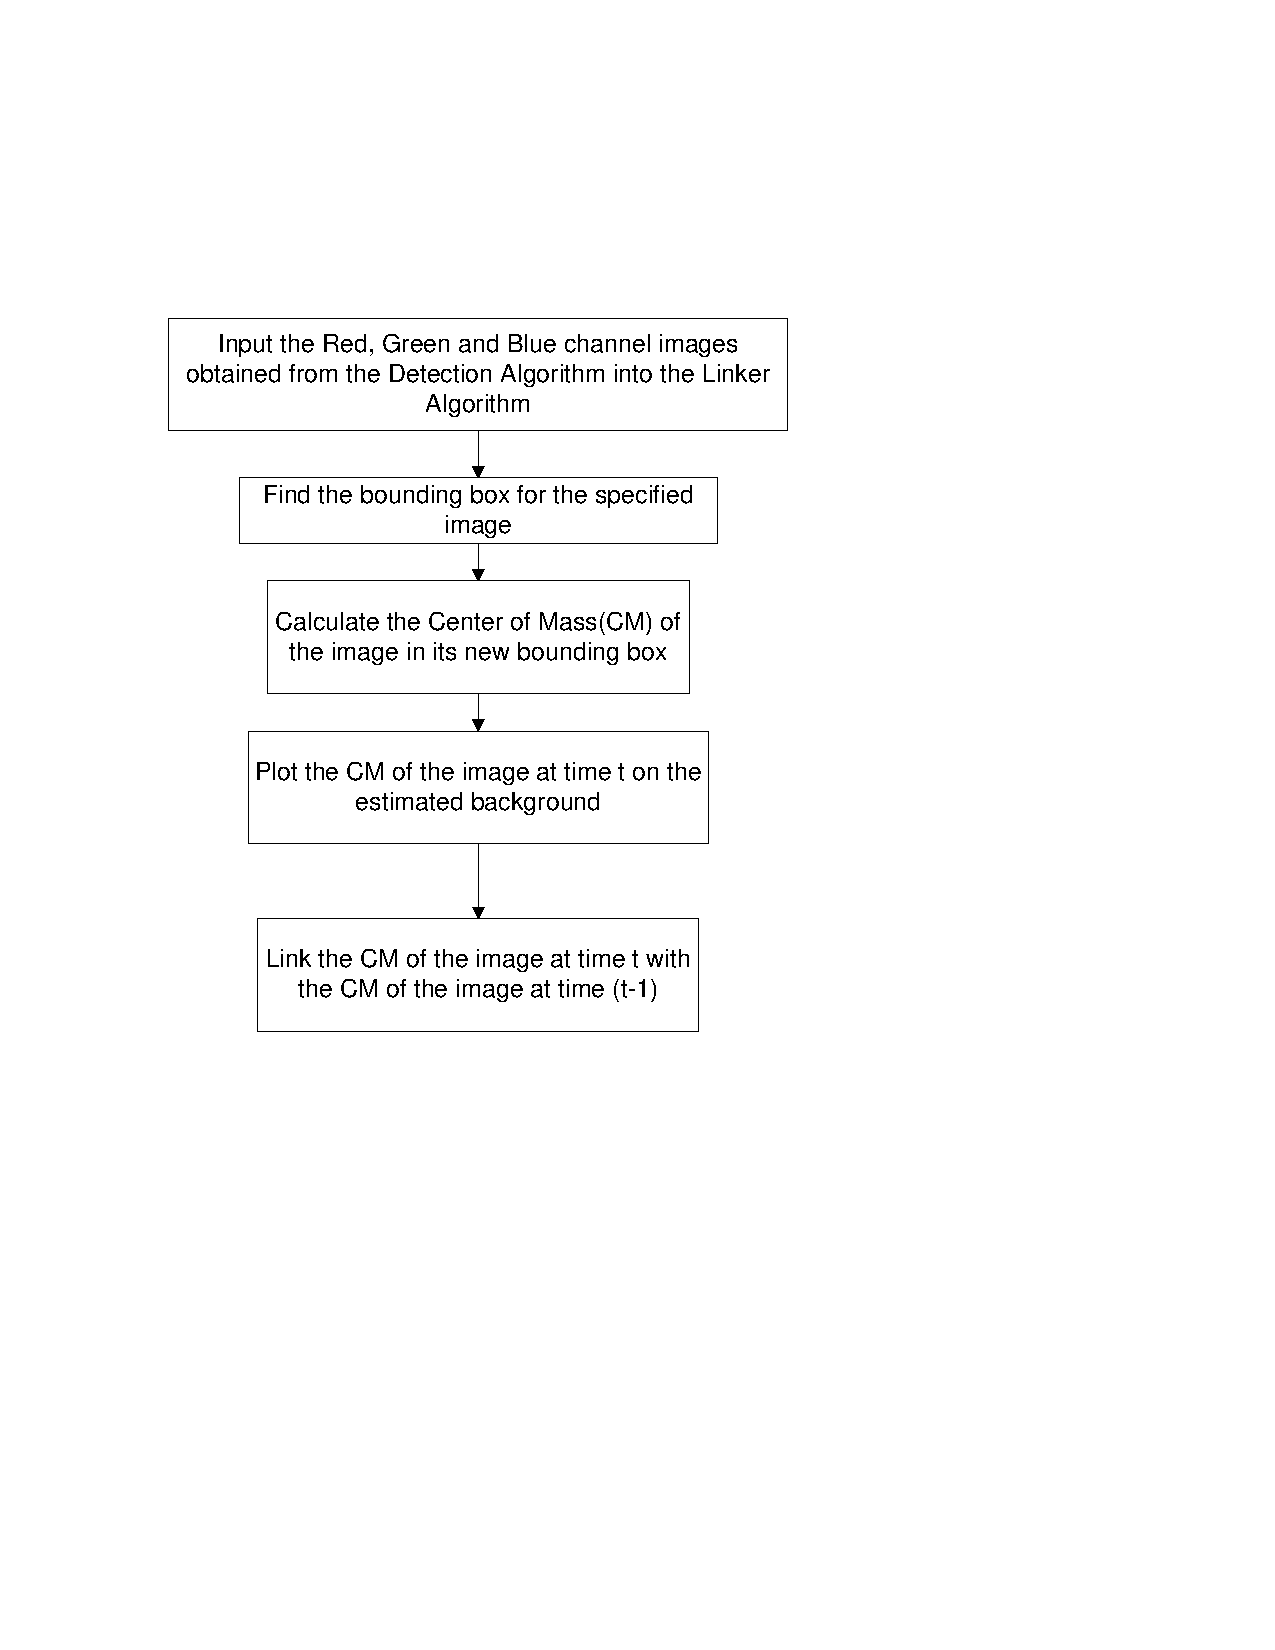
\includegraphics[width=0.5\textwidth]{../Drawings/linkingAlgorithm.pdf}
    \caption{The algorithm developed to link detections of the robot in consecutive frames}
    \label{fig:link}
\end{figure}


Once the images containing the robots have been received, a bounding box for each robot is calculated as well as the box's corresponding centroid. This is achieved in code using the `calcBoundingBox' function. This function has been developed according to \figref{fig:bounding}. Each image is labelled using the `mybwlabel' function. This will identify all of the objects in the image. The object with the largest area (I.e. the robot) will then be surrounded by its corresponding bounding box. The centroid of this bounding box is then calculated. This is performed on each of the three images corresponding to their repective colour channels.

\begin{figure}[h!] 
  \centering
    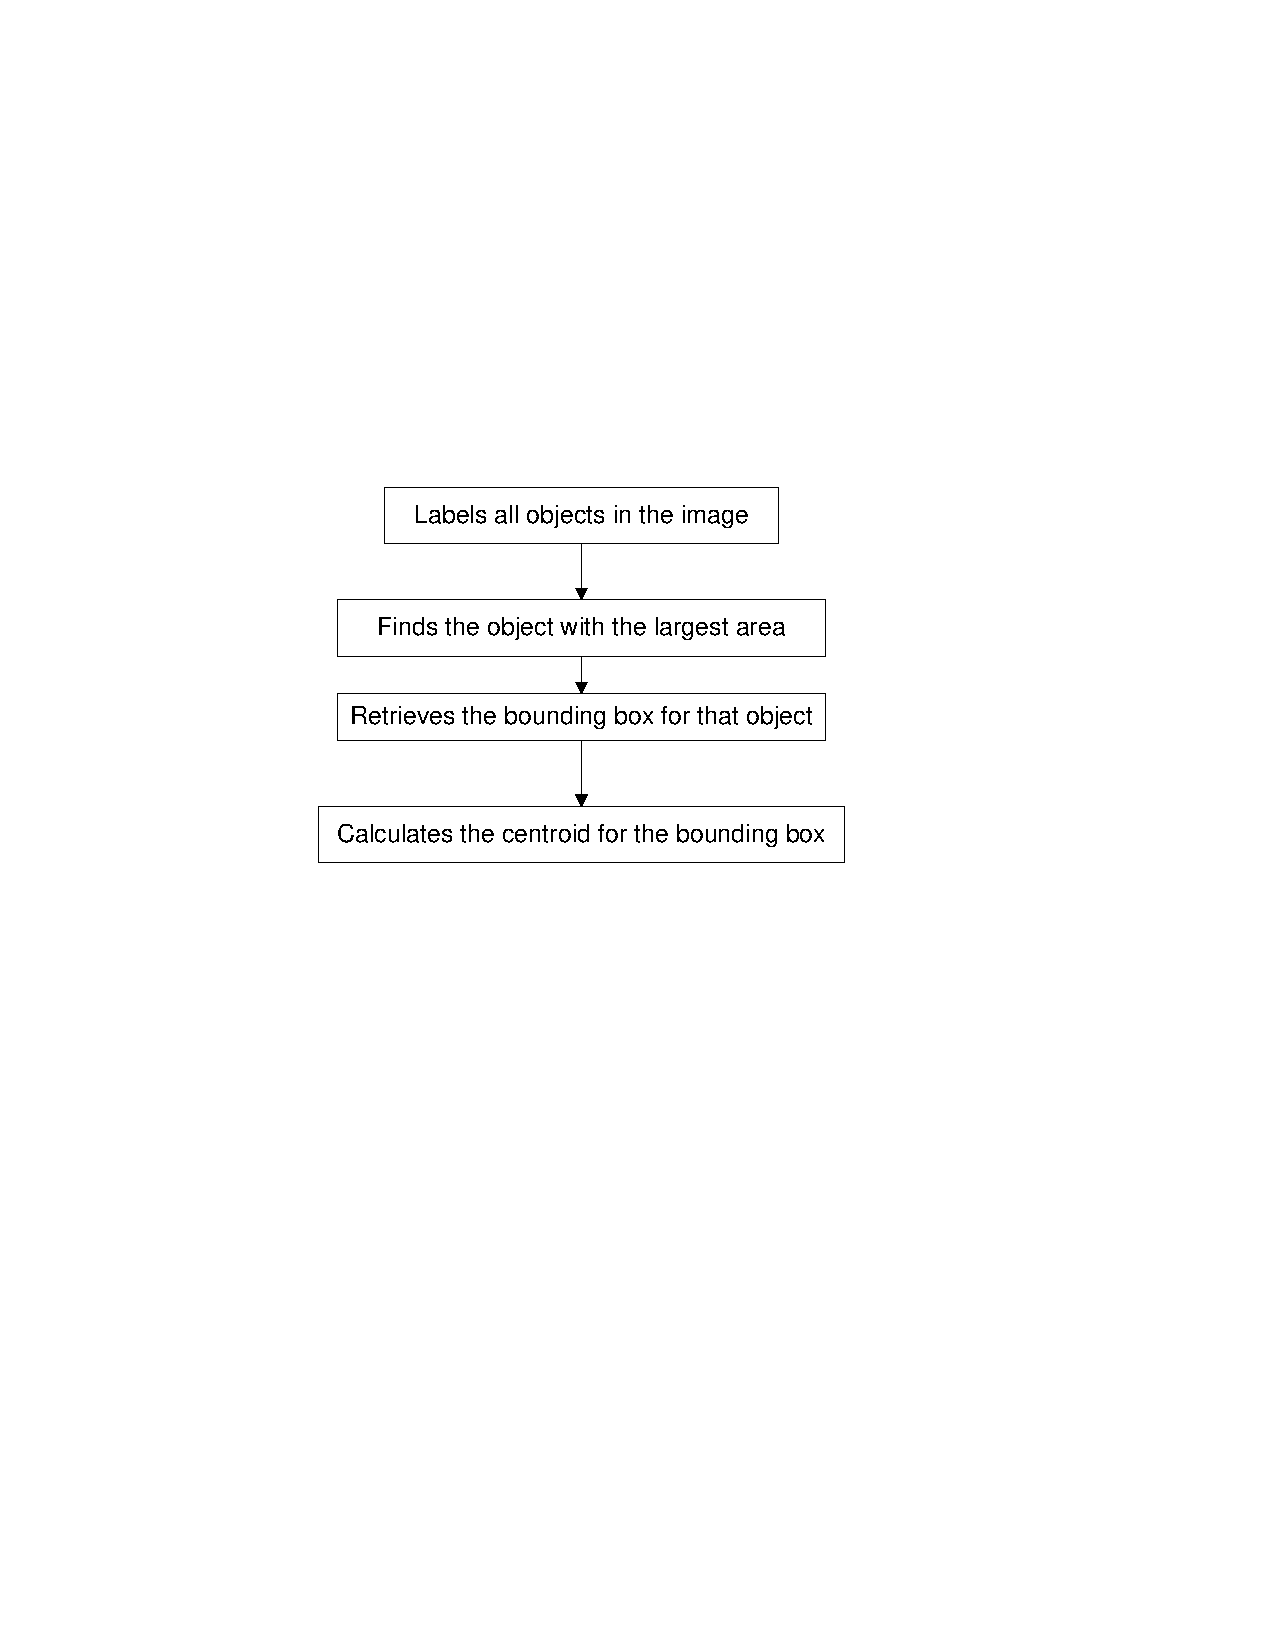
\includegraphics[width=0.5\textwidth]{../Drawings/boundingbox.pdf}
    \caption{The bounding box calculation for each robot }
    \label{fig:bounding}
\end{figure}

Once a bounding box for the robot has been determined, the center of mass of the robot needs to be calculated. This is achieved by utilising the `calcBoundingBoxCM' function.

This algorithm makes use of two important equations shown in \eqnref{eqn:area} and \eqnref{eqn:cm} respectively.

\begin{equation}
A = \Sigma_{r}\Sigma_{c}P_{rc}
\label{eqn:area}
\end{equation}

\begin{equation}
(\widehat{r}, \widehat{c}) = (\frac{1}{A}\Sigma_{r}\Sigma_{c}r P_{rc}, \frac{1}{A}\Sigma_{r}\Sigma_{c}c P_{rc})
\label{eqn:cm}
\end{equation}


\section{Results}
\label{sec:results}
%Test data

%Show an example of results for each stage of detection

\section{Discussion}
\label{sec:discussion}
%Assess the success of the program with regard to:

%1. Report results

%Discuss any
%1. Limitations, problems
%2. Improvements you would make

\section{Code}
\label{sec:code}
%Any downloaded code should be recorded in the report. Does not need to be in the appendix
%Code from course web pages are not needed

\section{Conclusion}
\label{sec:conclusion}

%\bibliographystyle{witseie}
%\bibliography{bibliography}
 \newpage
\onecolumn
\appendix
\setcounter{table}{0}
\setcounter{figure}{0}
\setcounter{subsection}{0}
\makeatletter \renewcommand{\thefigure}{A.\@arabic\c@figure} \renewcommand{\thetable}{A.\@arabic\c@table} \renewcommand{\thesection}{A.\@arabic\c@section} \makeatother
\section*{APPENDIX A}

\section{Control Program}
%Add the matlab code to this file...
%\lstinputlisting{codeSnippets.cpp}
 
\end{document}

